\documentclass{article}
\usepackage[utf8]{inputenc}
\usepackage[english,ngerman]{babel}
%% ========================================================================
%%%% MISC usepackages
%% ========================================================================

%% Chemistry
\usepackage{chemfig,chemmacros}
\chemsetup{modules = all}
\chemsetup[redox]{explicit-sign = true}
\chemsetup[phases]{pos=sub}
%\chemsetup[reactions]{before-tag = {R}, tag-open = [, tag-close = ]}
  
%% Maths
\usepackage{amsmath,amssymb,amsthm,textcomp}

%% Physics
\usepackage{siunitx}

%% Graphics
\usepackage{graphicx}
\usepackage{tikz}
\usepackage{rotating}
%\usepackage{subfig}

%% Tables and Lists
\usepackage{enumerate}
\usepackage{multicol}
\usepackage{geometry}
\usepackage{tabu}
\usepackage{listings}
\usepackage{tabularx}

%% Structures and Style
\usepackage{caption}
\usepackage{subcaption}
\usepackage{booktabs}
\usepackage{colortbl}

\usepackage{xcolor}
\usepackage{xfrac}
\usepackage[export]{adjustbox}[2011/08/13]

\usepackage{booktabs}
\usepackage{float}

\usepackage{fancyhdr}

%% Citing and Settings
\usepackage[backend=biber,
style=numeric,
backref=true, 
natbib=true, %% offering natbib-compatible commands
hyperref=true, %% using hyperref-package references
sorting= none,
doi=true,
maxcitenames=10,
maxbibnames=100,
citestyle=numeric
]{biblatex}

\addbibresource{references.bib}

\usepackage[toc,automake]{glossaries}
\include{abbrevations}
\makeglossaries

\usepackage[colorlinks=true,linkcolor=blue]{hyperref}

%% Figure settings
\renewcommand{\figurename}{Abbildung}
\renewcommand{\tablename}{Tabelle}
\renewcommand{\listfigurename}{Abbildungsverzeichnis}
\renewcommand{\listtablename}{Tabellenverzeichnis}

%% Commands chemistry

\NewChemState\ElPot{ symbol=E , subscript-pos=right , superscript= , unit=\volt}


%% ========================================================================
%%%% Document Information
%% ========================================================================

%% Title
\title{Elektrochemie \cite{Versuchsvorschrift}} % Title
\author{Autor: Florian \textsc{Kluibenschedl}} % Author name
\date{Bericht verfasst am: \today} % Date for the report

% Page style - headers
\pagestyle{fancy}
\fancyhf{}
\rhead{PR Allgemeine Chemie A - SS2019}
\lhead{Institut für Allgemeine Chemie - Universität Innsbruck}
\rfoot{Experiment 9 - Seite \thepage}

\begin{document}
  \renewtagform{reaction}[Rgl. ]{}{}
  
  \maketitle % Insert the title, author and date
  
  \begin{center}
    \begin{tabular}{r p{4cm}}
      Versuchsdurchführung am: & 05. März 2019\\ % Date the experiment was performed
      Gruppe, Matrikelnummer: & 3, 11805747 \\
      Lehrveranstaltung: & PR Allgemeine Chemie A \\
      Institut: & Allgemeine, Anorganische und Theoretische Chemie \\
      Assistent: & Pann Johann % Instructor/supervisor
    \end{tabular}
  \end{center}


  \begin{abstract}
    Elektrochemie ist eine vielseitige Disziplin in der Chemie mit vielen nützlichen Anwendungen. Um ein besseres Verständnis der Möglichkeiten zu erlangen, wurden vier elektrochemische Systeme näher untersucht.
    
    Die Standardpotentiale dreier galvanischer Zellen wurden bestimmt. Das Potential einer \ch{Pb\sld}/\ch{Pb(NO3)2\aq} (\SI[mode=text]{1.0}{M}) // \ch{Cu(NO3)2\aq} (\SI[mode=text]{1.0}{M})/\ch{Cu\sld} Zelle betrug \SI[separate-uncertainty]{0.512 \pm 0.003}{V} $(s=\num{\pm 0.0015})$. Das Potential einer \ch{Zn\sld}/\ch{Zn(NO3)2\aq} (\SI[mode=text]{1.0}{M}) // \ch{Pb(NO3)2\aq} (\SI[mode=text]{1.0}{M})/\ch{Pb\sld} Zelle betrug \SI[separate-uncertainty]{0.403 \pm 0.020}{V} $(s=\num{\pm 0.011})$ und das Potential einer \ch{Zn\sld}/\ch{Zn(NO3)2\aq} (\SI[mode=text]{1.0}{M}) // \ch{Cu(NO3)2\aq} (\SI[mode=text]{1.0}{M})/\ch{Cu\sld} Zelle war \SI[separate-uncertainty]{0.983 \pm 0.080}{V} $(s=\num{\pm 0.043})$. Eine Elektrolyse mit Kupferelektroden erlaubte die Bestimmung der Faraday-Konstante. Der Mittelwert der Messungen ergab eine Konstante von \SI[mode=text]{1.082d5}{\coulomb\per\mole}. Im Vergleich zum Literaturwert ist diese Konstante zu hoch, was jedoch durch Fehler beim Messvorgang, wie etwa Stromabfall, erklärt werden kann. Das Löslichkeitsprodukt von \ch{Cu(OH)2\sld} konnte zu \num{3.20e-19} bestimmt werden. Dieser zu große Wert weicht um eine Größenordnung vom Literaturwert (\num{4.8e-20} bei \SI[mode=text]{25}{\degreeCelsius} \cite{LoslichkeitWerteCUOH}) ab. Die Komplexbildungskonstante von \ch{[Cu(NH3)4]\pch[2]\aq} wurde bestimmt und beträgt \SI[mode=text, separate-uncertainty]{2.0 \pm 2.3 d14}{}. Auch dieser Wert ist im Vergleich zum Literaturwert (\num{1.1d13} bei \SI[mode=text]{25}{\degreeCelsius} \cite{KomplexFormation}) um eine Größenordnung zu groß. Als Gründe für diese Abweichungen werden Messfehler vermutet.
  \end{abstract}
  
  \pagebreak
  
  \section{Theoretische Grundlagen}
  
    \subsection{Motivation} \label{sec:Motivation}
      
      Redoxreaktionen kommen in beinahe allen Bereichen der Chemie vor. Auch in der Industrie werden Redoxreaktionen z. B. zur Herstellung wichtiger Chemikalien verwendet, wie etwa die Darstellung von \ch{NaOH} im Rahmen der Elektrolyse einer Kochsalzlösung \cite{NaOHDarstellung}. Ein tieferes Verständnis dieser Reaktionen ist somit absolut vonnöten. 
      
      Das physikalische Prinzip hinter den Redoxreaktionen ist die Übertragung von Elektronen, damit die Elemente stabilere Zustände erreichen. In der Spannungsreihe werden die Elemente nach ihrer Tendenz, Elektronen aufzunehmen klassifiziert. \\
      
      Anmerkung zur Angabe von Konstanten im Protokoll: um Probleme mit mathematischen Funktionen wie etwa dem Logarithmus bzw. der Exponentialfunktion zu vermeiden, werden alle Gleichgewichtskonstanten dimensionslos angegeben. Dazu werden alle Spezies im jeweiligen Massenwirkungsgesetz durch die Standardkonzentration ($c_{Standard} = \SI[mode=text]{1}{M}$) dividiert.
  
    \subsection{Ziel des Experiments}
    
      Auf Basis der obigen Überlegungen ist das Ziel, ein besseres Verständnis der Redoxchemie zu erhalten. Dabei werden zuerst die Potentiale dreier galvanischer Zellen bestimmt. Anschließend wird die Faraday-Konstante bestimmt, die für Elektrolyseprozesse von Bedeutung ist. Zum Abschluss werden das Löslichkeitsprodukt von \ch{Cu(OH)2\sld} und die Komplexbildungskonstante von \ch{[Cu(NH3)4]\pch[2]} bestimmt. Die erhaltenen Daten sollen mit den Literaturwerten verglichen werden. 
    
  \section{Experimenteller Teil}
  
    \subsection{Verwendete Materialien}
              
      \begin{table}[H]
        \centering
        \caption[Materialienliste, Quelle: Autor]{Auflistung der verwendeten Geräte und Chemikalien für alle beschriebenen Experimente}
        \label{tab:Materialien}
        
        \begin{tabular}{@{}ll|ll@{}}
          \toprule
            Geräte & Hersteller & Chemikalie & bezogen von \\ \midrule
            2 \SI[mode=text]{100}{\milli\litre} Bechergläser & DURAN & \SI[mode=text]{1.0}{M} \ch{Zn(NO3)2}-Lösung & Vorrat \\
            Magnetrührer & CAT M 6.1 & \SI[mode=text]{1.0}{M} \ch{Cu(NO3)2}-Lösung & Vorrat \\
            \SI[mode=text,separate-uncertainty]{25.000(45)}{\milli\litre} Vollpipette & BRAND & \SI[mode=text]{1.0}{M} \ch{Pb(NO3)2}-Lösung & Vorrat \\
            \SI[mode=text,separate-uncertainty]{25.000(75)}{\milli\litre} Bürette & BRAND & \SI[mode=text]{1.0}{M} \ch{KNO3}-Lösung & Vorrat \\
            Stromschlüssel &  & konz. \ch{HCl} & Vorrat \\
            Voltmeter & UNI-T UT61D & \SI[mode=text]{0.10}{M} \ch{CuSO4}-Lösung & Vorrat \\
            Netzgerät & RS Pro IPS 303A & \SI[mode=text]{0.10}{M} \ch{KOH}-Lösung & Vorrat \\ 
            Rührfische &  & \SI[mode=text]{1.0}{M} \ch{KOH}-Lösung & Vorrat \\ 
            Schleifpapier &  & \SI[mode=text]{1.0}{M} \ch{NH3}-Lösung & Vorrat  \\
             &  & deionisiertes Wasser & Vorrat  \\             
             &  & \ch{Cu}-Stab & Vorrat \\
             &  & \ch{Pb}-Stab & Vorrat \\ 
             &  & \ch{Zn}-Stab & Vorrat \\ \bottomrule
        \end{tabular}
      \end{table}
      
    \pagebreak
    
    \subsection{Untersuchung von elektrochemischen Zellen unter Standardbedingungen}
      
      Kupfer (\ElPot[superscript=0](\ch{Cu}){0.337}) ist ein edles Metall und kann von den unedleren Metallen Blei (\ElPot[superscript=0](\ch{Pb}){-0.126}) und Zink (\ElPot[superscript=0](\ch{Zn}){-0.763}) reduziert werden\footnote{die angegebenen Standardpotentiale wurden \cite[S. 881]{PhysicalChemistryAtkings} entnommen}. In diesem Experiment werden die Potentiale von drei galvanischen Zellen bestimmt: 
      
      \begin{center}
        (I): \ch{Pb\sld}/\ch{Pb(NO3)2\aq} (\SI[mode=text]{1.0}{M}) // \ch{Cu(NO3)2\aq} (\SI[mode=text]{1.0}{M})/\ch{Cu\sld}
          
        (II): \ch{Zn\sld}/\ch{Zn(NO3)2\aq} (\SI[mode=text]{1.0}{M}) // \ch{Pb(NO3)2\aq} (\SI[mode=text]{1.0}{M})/\ch{Pb\sld}
          
        (III): \ch{Zn\sld}/\ch{Zn(NO3)2\aq} (\SI[mode=text]{1.0}{M}) // \ch{Cu(NO3)2\aq} (\SI[mode=text]{1.0}{M})/\ch{Cu\sld}
      \end{center}
        
      Die zugehörigen Redoxgleichungen können wie folgt angegeben werden:
      
      \begin{reactions}
        Pb\sld{} + Cu\pch[2]\aq{} &-> Pb\pch[2]\aq{} + Cu\sld \\
        Zn\sld{} + Pb\pch[2]\aq{} &-> Zn\pch[2]\aq{} + Pb\sld \\
        Zn\sld{} + Cu\pch[2]\aq{} &-> Zn\pch[2]\aq{} + Cu\sld
      \end{reactions}
      
      Da alle Reaktanden in Standardkonzentration vorliegen ($c_{i} = \SI[mode=text]{1}{M}$), können die gemessen Potentiale mit den theoretischen Standardpotentialen, die aus Literaturwerten errechnet wurden, direkt verglichen werden. Die theoretischen Standardpotentiale der Reaktionen können dabei wie in \eqref{eq:LiteraturStandard} angeführt berechnet werden. 
      
      \begin{equation}
        \ElPot*[superscript=0](Lit.){} = \ElPot*[superscript=0](Red.){} - \ElPot*[superscript=0](Ox.){} \label{eq:LiteraturStandard}
      \end{equation}
      
      Die Nernstgleichung \eqref{eq:Nernst}\footnote{$R = \SI[mode=text]{8.314}{\joule\per\mole\per\kelvin}, F = \SI[mode=text]{96485}{\ampere\second\per\mole}, z = $ Anzahl an übertragenen Elektronen, $Q = $ Massenwirkungsgesetz nicht im Gleichgewicht \cite{PhysicalChemistryAtkings}} gibt einerseits die Abhängigkeit des Potential von Temperatur und Konzentration der beteiligten Spezies an. Andererseits eignet sie sich, um die Gleichgewichtskonstante einer Redoxreaktion zu berechnen. 
        
      \begin{equation}
        \ElPot*[](){} = \ElPot*[superscript=0](Lit.){} - \frac{R * T}{z * F} * \ln Q \label{eq:Nernst}
      \end{equation}
      
      Die Gibbs Energie kann aus \ElPot*[](){} berechnet werden ($\gibbs*[superscript=](){} = - z * F * \ElPot*[](){}$). Im Gleichgewicht ($Q = K$) ist \gibbs[superscript=](){0} $\Rightarrow$ \ElPot[](){0}. Eingesetzt in die Nernstgleichung kann nun durch umformen die Gleichgewichtskonstante berechnet werden:
      
      \begin{equation}
        K = e^{\frac{z F}{R T} * \ElPot*[superscript=0](Lit.){}} \label{eq:Gleichgewichtskonstante}
      \end{equation}
      
      \subsubsection{Versuchsdurchführung} \label{sec:VersuchZellen}
        
        Zunächst wurden die jeweiligen Metallelektroden (Kupfer-, Zink- und Bleistab) mit Schleifpapier gesäubert\footnote{um eine etwaige Oxidschicht, Fett sowie anderen Schmutz zu entfernen} und anschließend etwas konz. \ch{HCl} gereinigt. Je ein Becherglas wurde mit ca. \SI[mode=text]{30}{\milli\liter} einer \SI[mode=text]{1.0}{M} Salzlösung befüllt. Die verwendeten Salzlösungen sind oben beschrieben. Der Stromschlüssel wurde mit \SI[mode=text]{1.0}{M} \ch{KNO3}-Lösung unter Vermeidung von Luftblasen befüllt und in die beiden als Halbzellen fungierenden Bechergläser gestellt\footnote{es wurde darauf geachtet, dass er in beide Lösungen ungefähr gleich tief eintauchte}. Das Voltmeter wurde an die beiden Metallelektroden angeschlossen. Diese wurden jeweils in ein Becherglas mit zugehöriger Salzlösung gestellt. Nachdem sich der Messwert stabilisiert hatte (ca. \SI[mode=text]{5}{\second}), wurde er abgelesen. 
        
        Die Messung der Potentialdifferenzen wurde pro galvanischer Zelle dreimal wiederholt, wobei die Metallelektroden zwischen jeder Messung wie oben beschrieben gründlich gesäubert wurden, um unerwünschte kinetische Effekte an den Oberflächen möglichst zu vermeiden.      
      
      \subsubsection{Messergebnisse und Literaturwerte}
    
        In Tabelle \ref{tab:MessdatenPotentialdifferenzenZellen} sind alle Messwerte aufgelistet, die im Rahmen der Versuchsdurchführung wie in \ref{sec:VersuchZellen} beschrieben, gemessen wurden. 
      
        \begin{table}[H]
          \centering
          \caption[Messdaten, Quelle: Autor]{Messdaten}
          \label{tab:MessdatenPotentialdifferenzenZellen}
            \begin{tabular}{@{}l|l|l@{}}
              \toprule
               \ElPot*[superscript=0]($\ch{Pb}/\ch{Pb\pch[2]}//\ch{Cu\pch[2]}/\ch{Cu}$){} in V & \ElPot*[superscript=0]($\ch{Zn}/\ch{Zn\pch[2]}//\ch{Pb\pch[2]}/\ch{Pb}$){} in V & \ElPot*[superscript=0]($\ch{Zn}/\ch{Zn\pch[2]}//\ch{Cu\pch[2]}/\ch{Cu}$){} in V \\ \midrule
               0.511 & 0.414 & 0.973  \\
               0.514 & 0.393 & 0.946  \\
               0.512 & 0.401 & 1.031  \\ \bottomrule
            \end{tabular}
         \end{table}      
      
      \subsubsection{Ergebnisse und Diskussion} \label{sec:ErgebnissePotentialeEins}
      
      In Tabelle \ref{tab:MessdatenPotentialdifferenzenZellenlit} werden die aus \ref{tab:MessdatenPotentialdifferenzenZellen} errechneten, gemessenen Standardpotentiale aufgelistet und mit den zugehörigen Literaturwerten verglichen. Die angegebenen thermodynamischen Gleichgewichtskonstanten wurden aus den Literaturwerten und gemessenen Potentialen nach \eqref{eq:Gleichgewichtskonstante} berechnet und zeigen, dass das Gleichgewicht aller drei Reaktionen stark auf Seite der Produkte liegt.
      
      \begin{table}[H]
        \centering
        \caption[Messdaten und Vergleiche mit der Literatur, Quelle: Autor]{Messdaten und Literaturwerte - $T_{Exp.}=\SI[mode=text]{22}{\degreeCelsius}$}
        \label{tab:MessdatenPotentialdifferenzenZellenlit}
          \begin{tabular}{@{}l|l|lll@{}}
            \toprule
             Zelle & \ElPot*[superscript=0](exp.){} in V - $\alpha=0.05,N=3$ & \ElPot*[superscript=0](Lit.){} in V & $K_{Lit.}$ & $K_{Exp.}$ \\ \midrule
             $\ch{Pb}/\ch{Pb\pch[2]}//\ch{Cu\pch[2]}/\ch{Cu}$ & \num[separate-uncertainty]{0.512 \pm 0.003} $(s=\num{\pm 0.0015})$ & 0.463 & \num{4.58e15} & \num{3.13e17}\\
             $\ch{Zn}/\ch{Zn\pch[2]}//\ch{Pb\pch[2]}/\ch{Pb}$ & \num[separate-uncertainty]{0.403 \pm 0.020} $(s=\num{\pm 0.011})$ & 0.637 & \num{3.52e21} & \num{5.89e13}\\
             $\ch{Zn}/\ch{Zn\pch[2]}//\ch{Cu\pch[2]}/\ch{Cu}$ & \num[separate-uncertainty]{0.983 \pm 0.080} $(s=\num{\pm 0.043})$ & 1.10 & \num{1.62e37} & \num{3.88e33}\\ \bottomrule
         \end{tabular}
      \end{table} 
      
      Wie aus der Tabelle ersichtlich, unterscheiden sich die gemessenen Werte der Potentiale doch recht stark von den Literaturwerten.  Gründe für diese Abweichungen sollen im Folgenden diskutiert werden. Die Messung der Blei-Kupfer Zelle war jene mit der höchsten Präzision\footnote{kleinste Standardabweichung} und geringsten Abweichung vom Literaturwert. Die Messungen der Zink-Blei Zelle und der Zink-Kupfer Zelle lieferten beide niedrigere Werte. \\ 
      
      Eine Erklärung für diese Beobachtungen könnten unterschiedliche Konzentrationen der vorgelegten Salzlösungen sein. Sind diese nämlich nicht \SI[mode=text]{1.0}{M}, so können die unterschiedlichen Werte mit der Nernstgleichung - \eqref{eq:Nernst} - erklärt werden. Der höhere Potentialwert für die Blei-Kupfer Zelle kann durch eine niedrigere Bleikonzentration erklärt werden bei entweder größerer Kupferkonzentration oder Kupferkonzentration von \SI[mode=text]{1.0}{M}. Die niedrigere Bleikonzentration würde bei entweder größerer Zinkkonzentration oder Zinkkonzentration von \SI[mode=text]{1.0}{M} auch das niedrigere Potential der Zink-Blei Zelle erklären. Eine größere Zinkkonzentration widerum würde den geringeren Potentialwert der Zink-Kupfer Zelle erklären. Die Kupferkonzentration müsste damit entweder \SI[mode=text]{1.0}{M}, kleiner oder größer, aber nicht größer wie jene von Zink sein. 
      
      In diesem Sinne könnte eine niedrigere Blei-, größere Zinkkonzentration und größere Kupferkonzentration\footnote{nach unten durch 1 und nach oben durch die Zinkkonzentration beschränkt} die Abweichungen erklären. Ein Grund für das Zustandekommen der abweichenden Konzentrationen könnte sein, dass durch die nach Gebrauch wieder zurückgeleerten Lösungen der Studenten Verunreinigungen, zusätzliches Wasser, ... eingebracht wurden. Grundsätzlich kann aber, denke ich, schon davon ausgegangen werden, dass die Konzentrationen stimmen. \\
      
      Beim Säubern der Elektroden wurde beobachtet, dass die Bleielektroden sich am schlechtesten reinigen ließen. Von einer unreineren Elektrode können die Elektronen auf das zu reduzierende Blei-(II)-Ion nicht so gut übertragen werden. Dies könnte die kleinere Gleichgewichtskonstante und damit das geringere Potential der Zink-Blei Zelle erklären. Die Blei-Halbzelle hätte damit ein effektiv negativeres Potential, was auch das größere Potential der Blei-Kupfer Zelle erklären könnte. 
      
      Ansonsten können diverse kinetische Hemmungen an den Oberflächen der Elektroden als Erklärung für die Abweichungen herangezogen werden. In dieser Hinsicht hat vielleicht auch die unterschiedliche (große) Oberfläche der Elektroden einen Einfluss. \\
      
      Des weiteren ist zu berücksichtigen, dass die Literaturwerte für \SI[mode=text]{25}{\degreeCelsius} angegeben werden, die Messungen jedoch bei etwa \SI[mode=text]{22}{\degreeCelsius} durchgeführt wurden\footnote{die Temperatur wurde bei den Messungen nicht explizit gemessen, kann jedoch durch den Erfahrungswert des vorherigen Praktikumstag abgeschätzt werden}. \\
      
      Um die Messergebnisse zu verbessern, wird an dieser Stelle folgendes vorgeschlagen: 
      
      \begin{itemize}
        \item saubere Messapparatur mit Halterungen für die Elektroden aufzubauen
        \item Verwendung von Elektroden mit gleicher Oberfläche
        \item vor Messung eine titrimetrische Überprüfung der Konzentrationen der Salzlösungen durchzuführen
        \item Messungen bei \SI[mode=text]{25}{\degreeCelsius} durchzuführen
      \end{itemize}
    
    \pagebreak
    
    \subsection{Elektrolyse - Bestimmung der Faraday Konstante}
    
      Bisher wurden elektrochemische Systeme betrachtet, die freiwillig ablaufen. Die oben beschriebenen galvanischen Zellen eignen sich somit unter anderem, um Batterien zu bauen, da sie unter Abgabe von Energie reagieren. Bei der Elektrolyse findet genau der umgekehrte Prozess statt. Es wird nun Energie, also Strom benötigt, um eine elektrochemische Reaktion aufrecht zu erhalten. 
      
      Die in einem bestimmten Zeitintervall übertragene Ladungsmenge $Q$ kann wie in \eqref{eq:Q} dargestellt aus dem zeitlichen Integral des Stromes berechnet werden, da dieser als Änderung der Ladung in einer bestimmten Zeit definiert ist ($I=\frac{dQ}{dt}$). Zusätzlich ist die Ladungsmenge proportional zur Anzahl der übertragenen Elektronen $z * n$ ($n$ ist die Stoffmenge in mol). Der Proportionalitätsfaktor wird mit $F$ bezeichnet.
      
      \begin{equation}
        Q = I \int_{0}^{t} dt = I * t = z * F * n = z * F * \frac{m}{M} \label{eq:Q}
      \end{equation}
      
      Durch Umstellen kann die sogenannte Faraday-Konstante $F$ berechnet werden:
      
      \begin{equation}
        F = \frac{I * t * M}{z * m} \label{eq:Faraday}
      \end{equation}
      
      Wird nun über eine bestimmte Zeit ein bekannter Strom angelegt, kann durch Messung der Massendifferenz die Faraday-Konstante bestimmt werden. Im Folgenden wird eine Elektrolyse mit Kupferelektroden und einer \ch{CuSO4} Lösung betrachtet. 
      
      \subsubsection{Versuchsdurchführung}
        
        \begin{figure}[h]
          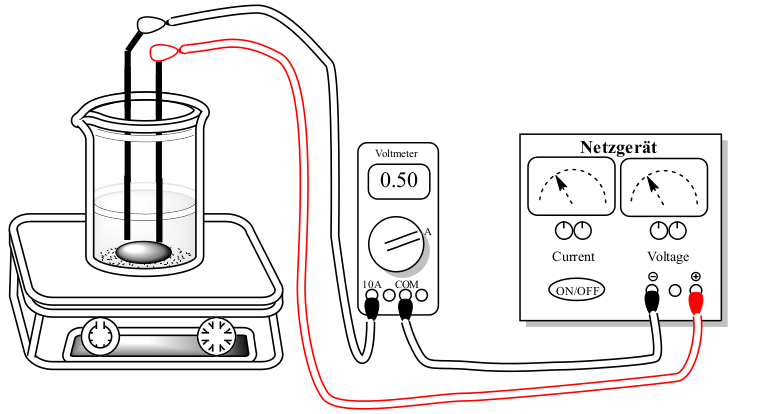
\includegraphics[scale=0.4, center]{Graphiken/Versuchsanordnungen/ElektrolyseAufbau.png} 
          \caption[schematische Versuchsanordnung Bestimmung der Faraday-Konstante, Quelle: \cite{Versuchsvorschrift}]{schematische Versuchsanordnung der Elektrolyse \cite{Versuchsvorschrift}}
          \label{fig:Versuchsanordnung}
        \end{figure}
    
        Zu Beginn wurde der Strom am Messgerät auf ca. \SI[mode=text]{0.5}{\ampere} eingestellt. Dazu wurde ein Kurzschluss herbeigeführt, um auf Strombegrenzung zu schalten. Im Anschluss wurde der Strom eingestellt. 
        
        Der Versuch wurde wie in Abbildung \ref{fig:Versuchsanordnung} gezeigt aufgebaut. Das Strommessgerät wurde dazu seriell in den Stromkreis eingebaut, um die Messung bzw. Regulierung des exakten Stromes zu ermöglichen. Die beiden Kupferelektroden wurden mit Krokodilklemmen wie beschrieben angeschlossen. Als Elektrolytlösung wurden ca. \SI[mode=text]{50}{\milli\liter} einer \SI[mode=text]{1.0}{M} \ch{CuSO4}-Lösung in einem \SI[mode=text]{100}{\milli\liter} Becherglas verwendet. Die Elektroden wurden mit Schleifpapier gesäubert und in \SI[mode=text]{4}{M} \ch{HCl} gewaschen. Eine der Kupferelektroden wurde durch Biegung markiert. Die Elektroden wurden für ca. \SI[mode=text]{2}{\minute} im Trockenschrank bei ca. \SI[mode=text]{120}{\degreeCelsius} getrocknet. Nach dem Abkühlen wurden sie abgewogen und in das Becherglas gestellt. Es wurde darauf geachtet, dass sich die beiden Elektroden während der Elektrolyse nicht gegenseitig berühren\footnote{dazu diente eine kleine Styroporplatte als Abstandshalter}. Nachdem der Versuch vollständig wie beschrieben aufgebaut war, wurde der Strom eingeschalten und die Zeitmessung gestartet. Nach ca. \SI[mode=text]{10}{\minute} wurde die Elektrolyse abgebrochen, die Kupferelektroden entnommen, mit deionisiertem Wasser gespült und für ca. \SI[mode=text]{2}{\minute} im Trockenschrank bei ca. \SI[mode=text]{120}{\degreeCelsius} getrocknet. Nach dem Abkühlen wurde wieder abgewogen. 
        
      \subsubsection{Messergebnisse} \label{sec:MessergebnisseFaraday}
      
        \begin{table}[H]
          \centering
          \caption[Messdaten der Bestimmung der Faraday Konstante, Quelle: Autor]{Messdaten}
          \label{tab:MessdatenFaraday}
            \begin{tabular}{@{}l|ll@{}}
              \toprule
                & Anode & Kathode \\ \midrule
               $m_{vorher}$ in g & 5.987 & 6.689 \\
               $m_{nachher}$ in g & 5.906 & 6.787 \\
               $\Delta m$ in g & -0.081 & 0.098 \\ \bottomrule
            \end{tabular}
        \end{table}
        
        Das Netzgerät wurde anfangs auf \SI[mode=text]{0.496}{\ampere} und \SI[mode=text]{3}{\volt} eingestellt - näheres siehe \ref{sec:ErgebnisseFaraday}. Gemessen wurde für \SI[mode=text]{10.1}{\minute}. $M_{\ch{Cu}}=\SI[mode=text]{63.54}{gram\per\mole}$
        
      \subsubsection{Ergebnisse und Diskussion} \label{sec:ErgebnisseFaraday}
      
        Werden die in \ref{sec:MessergebnisseFaraday} angegebenen Werte in \eqref{eq:Faraday} eingesetzt, ergeben sich folgende Werte für die Faraday-Konstante: $F_{Anode} = \SI[mode=text]{1.185d5}{\coulomb\per\mole}$, $F_{Kathode} = \SI[mode=text]{9.792d4}{\coulomb\per\mole}$, $F_{Mittelwert} = \SI[mode=text]{1.082d5}{\coulomb\per\mole}$. Ein Vergleich mit dem Literaturwert ($F = \SI[mode=text]{96485.309}{\coulomb\per\mole}$ \cite{Faraday}) zeigt, dass die aus der Massenzunahme ermittelte Faradaykonstante dem Literaturwert am nächsten kommt. Die zu hohe Konstante, die sich aus der geringeren Massenabnahme der Anode errechnet und der daraus resultierende hohe Mittelwert der beiden Messwerte bedarfen einer Erklärung. \\
        
        Angenommen, die komplette Versuchsdurchführung war von keinen Fehlern begleitet. Eine Erklärung für die geringere Massenabnahme der Anode könnte sein, dass als Parallelreaktion zur Oxidation von Kupfer die Oxidation von Wasser zu Sauerstoff ablief. Eine charakteristische Bläschenbildung konnte jedoch nicht beobachtet werden, weswegen diese Erklärung wegfällt. 
        
        Während der Elektrolyse wurde zweimal ein Stromabfall bemerkt - einmal auf ca. \SI[mode=text]{0.44}{\ampere} und ein zweites Mal auf ca. \SI[mode=text]{0.35}{\ampere}. Nach dem Stromabfall wurde wieder auf ca. \SI[mode=text]{0.5}{\ampere} eingestellt. Der für einige Zeit geringere Stromfluss bedeutet, dass in dieser Zeit der Reaktionsumsatz geringer war. Dies würde die größere Faraday-Konstante erklären. Allerdings erklärt der Stromabfall nicht, warum die Massenzunahme der Kathode deutlich größer ist wie der Betrag der Massenabnahme der Anode. Dass die aus der Massenzunahme der Kathode berechnete Faraday-Konstante mit dem Literaturwert recht gut übereinstimmt, zeigt, dass der beobachtete Stromabfall nicht allzu große Auswirkungen auf das Ergebnis hatte. Er erklärt den leicht zu großen Wert von $F_{Kathode}$.
        
        Am wahrscheinlichsten ist ein Mess- oder sogar Ablesefehler beim Abwiegen der Anode nach dem Trocknen. Wurde die Anode bei zu hoher Temperatur abgewogen, könnte der Auftrieb der heißen Luft die geringere Massendifferenz erklären. Auch könnten durch das Berühren mit den Fingern Fettreste, ... auf die Anode aufgebracht worden sein. \\
        
        Um die Messergebnisse zu verbessern, wird an dieser Stelle folgendes vorgeschlagen: 
      
      \begin{itemize}
        \item die beiden Elektroden besser befestigen - stabile Halterung
        \item spröde bzw. brüchig erscheinende Elektroden sofort ersetzen
        \item die Stabilität des Netzgerätes im Vorfeld für ein paar Minuten testen
        \item bessere Handhabung der Waage 
      \end{itemize}
        
    \pagebreak
    
    \subsection{Bestimmung des Löslichkeitsproduktes von \ch{Cu(OH)2\sld}}
      
      \ch{Cu(OH)2\sld} löst sich wie in \ref{rec:LosungCUOH} beschrieben. Das Löslichkeitsprodukt berechnet sich wie in \eqref{eq:Loslichkeitprodukt} angeführt.  
      
      \begin{reaction}
        Cu(OH)2\sld{} <<=> Cu\pch[2]\aq{} + 2 OH\mch\aq{} \label{rec:LosungCUOH}      
      \end{reaction}
      
      \begin{equation}
        K_{L} = [\ch{Cu\pch[2]\aq}] * [\ch{OH\mch\aq}]^2 \label{eq:Loslichkeitprodukt}
      \end{equation}
      
      Ist  die Konzentration von \ch{OH\mch\aq} im Gleichgewicht bekannt, kann durch Messen von [\ch{Cu\pch[2]\aq}] das gesuchte Löslichkeitsprodukt berechnet werden. Dazu wurde die folgende galvanische Zelle verwendet:
      
      \begin{center}
        \ch{Cu\sld}/\ch{Cu(OH)2\sld},\ch{OH\mch\aq} // \ch{Cu\pch[2]\aq} (\SI[mode=text]{0.10}{M})/\ch{Cu\sld}
      \end{center}
      
      Die Spannung dieser Zelle kann mithilfe der Nernstgleichung berechnet werden. Da es sich um eine sogenannte Konzentrationszelle handelt\footnote{bei einer Konzentrationszelle wird die Redoxreaktion nur durch einen Konzentrationsunterschied hervorgerufen}, ist \ElPot[superscript=0](){0} und die Nernstgleichung vereinfacht sich zu:
      
      \begin{equation}
        \ElPot*[](){} = - \frac{R * T}{z * F} * \ln \frac{[\ch{Cu\pch[2]\aq}]_{Anode}}{[\ch{Cu\pch[2]\aq}]_{Kathode}} \label{eq:Elpot}
      \end{equation}
      
      Die Konzentration von \ch{Cu\pch[2]} im Kathodenraum ist bekannt ($[\ch{Cu\pch[2]\aq}]_{Kathode} = \SI[mode=text]{0.10}{M}$). Durch umformen von \ref{eq:Elpot} erhält man einen Ausdruck, mit dem die Konzentration von \ch{Cu\pch[2]} im Anodenraum berechnet werden kann:
      
      \begin{equation}
        [\ch{Cu\pch[2]\aq}]_{Anode} = [\ch{Cu\pch[2]\aq}]_{Kathode} * e^{- \frac{\ElPot*[](){} * z * F}{R * T}} 
      \end{equation} \\
      
      Nun kann das gesuchte Löslichkeitsprodukt berechnet werden:
      
      \begin{equation}
        K_{L} = [\ch{Cu\pch[2]\aq}]_{Kathode} * e^{- \frac{\ElPot*[](){} * z * F}{R * T}} * [\ch{OH\mch\aq}]^2 \label{eq:Loslichkeitsproduktfinale}
      \end{equation}
      
      \subsubsection{Versuchsdurchführung} \label{sec:VersuchsdurchfuhrungLoslichkeit}
      
      Je ein \SI[mode=text]{100}{\milli\liter} Becherglas wurde mit \SI[mode=text]{50}{\milli\liter} einer \SI[mode=text]{0.10}{M} \ch{CuSO4} bzw. \SI[mode=text]{50}{\milli\liter} einer \SI[mode=text]{0.10}{M} \ch{KOH}. Als Stromschlüssel wurde derselbe wie in \ref{sec:VersuchZellen} verwendet. Dieser wurde in etwa gleich tief in beide Bechergläser eingetaucht. Zwei \ch{Cu}-Elektroden wurden mit Schleifpapier und konz. \ch{HCl} gereinigt und mit deionisiertem Wasser gespült\footnote{um keine störenden Ionen in die Zelle zu bringen}. Nach dem Trocknen wurden sie an das Voltmeter angeschlossen und in die beiden Bechergläser getaucht. Die Spannung wurde unmittelbar nach dem Eintauchen in die Lösung gemessen und notiert, da es durch Polarisationseffekte sehr schnell zur Spannungsänderung kommt. Es wurden zwei weitere Messungen nach dem gleichem Prinzip durchgeführt.
      
      Anschließend wurde die oben beschriebene Messung mit \SI[mode=text]{1.0}{M} \ch{KOH} durchgeführt. 
      
      \subsubsection{Messergebnisse}
      
        \begin{table}[H]
          \centering
          \caption[Messdaten der Bestimmung des Löslichkeitsproduktes, Quelle: Autor]{Messdaten}
          \label{tab:MessdatenPotentialLoslichkeit}
            \begin{tabular}{@{}l|l@{}}
              \toprule
               \ElPot*[superscript=0]($\ch{Cu}/\ch{Cu(OH)2}//\ch{Cu\pch[2]}/\ch{Cu}$){} in V für \SI[mode=text]{0.1}{M} \ch{KOH} & \ElPot*[superscript=0]($\ch{Cu}/\ch{Cu(OH)2}//\ch{Cu\pch[2]}/\ch{Cu}$){} in V für \SI[mode=text]{1}{M} \ch{KOH} \\ \midrule
               0.396 & 0.498 \\
               0.401 & 0.512 \\
               0.410 & 0.525 \\ \bottomrule
            \end{tabular}
        \end{table}
         
      \subsubsection{Ergebnisse und Diskussion}
      
        \begin{table}[H]
          \centering
          \caption[Messergebnisse der Bestimmung des Löslichkeitsproduktes, Quelle: Autor]{Messergebnisse und daraus errechnete Größen - $T=\SI[mode=text]{22}{\degreeCelsius}$}
          \label{tab:MessdatenPotentialLoslichkeitErgebnisse}
            \begin{tabular}{@{}l|lll@{}}
              \toprule
                & \ElPot*[superscript=0]($\ch{Cu}/\ch{Cu(OH)2}//\ch{Cu\pch[2]}/\ch{Cu}$){} in V  & $[\ch{Cu\pch[2]\aq}]_{eq.}$ in M & $K_{L}$ \\ \midrule
               \SI[mode=text]{0.1}{M} \ch{KOH} & \num[separate-uncertainty]{0.402 \pm 0.013} $(s=\num{\pm 0.0071},\alpha=0.05,N=3)$ & \num{1.84e-15} & \num{1.84e-17} \\
               \SI[mode=text]{1}{M} \ch{KOH} & \num[separate-uncertainty]{0.512 \pm 0.026} $(s=\num{\pm 0.014},\alpha=0.05,N=3)$ & \num{3.20e-19} & \num{3.20e-19}  \\ \bottomrule
            \end{tabular}
        \end{table}
        
        Im Vergleich zum Literaturwert des Löslichkeitsproduktes (\num{4.8e-20} bei \SI[mode=text]{25}{\degreeCelsius} \cite{LoslichkeitWerteCUOH}) ist der gemessene Wert bei Verwendung der \SI[mode=text]{0.10}{M} \ch{KOH} um 3 Größenordnungen zu hoch. Der gemessene Wert bei Verwendung der \SI[mode=text]{1.0}{M} \ch{KOH} war nur mehr um 1 Größenordnung zu groß. Die Präzision beider Messungen liegt in einem annehmbaren Rahmen und ist vergleichbar mit den in \ref{sec:ErgebnissePotentialeEins} notierten. 
        
        Die größere \ch{OH\mch\aq} Konzentration hat zur Folge, dass gemäß der Formel für das Löslichkeitsprodukt die \ch{Cu\pch[2]\aq} Konzentration kleiner wird. Eine kleinere \ch{Cu\pch[2]\aq} Konzentration bewirkt nun, wie man mit der Nernstgleichung sieht, ein größeres Potential. Messtechnisch gesehen müsste eine größere Spannung besser zu messen sein. Das Problem bei dieser Erklärung ist jedoch, dass die Präzision bei höherer Spannung abnahm. Dennoch kann so erklärt werden, dass bei größerer \ch{OH\mch} Konzentration das experimentelle Löslichkeitsprodukt dem theoretischen näher kommt. Zu beachten ist jedoch, dass bei höherer Konzentration ab einem gewissen Punkt nicht mehr mit Konzentrationen gerechnet werden kann. \\
        
        Eine weitere Fehlerquelle könnte eine fehlerhafte Ablese der Werte sein. Da die Elektroden sehr schnell polarisiert werden, änderte sich die gemessene Spannung sehr schnell. Es wurde zwar versucht, den ersten einigermaßen stabilen Messwert (nach ca. \SI[mode=text]{3}{\second}) zu notieren, was aber aufgrund der Schwankungen recht schwierig war.
        
        Um die Messergebnisse zu verbessern, wird an dieser Stelle folgendes vorgeschlagen: 
      
        \begin{itemize}
          \item größere \ch{KOH}-Konzentrationen zu verwenden
          \item eine stabile Messapparatur mit Halterungen aufzubauen
        \end{itemize}
     
      \pagebreak
        
      \subsection{Bestimmung der Komplexbildungskonstante von \ch{[Cu(NH3)4]\pch[2]}}
        
        Kupfer reagiert mit Ammoniak unter Bildung eines Tetramminkupfer-(II) Komplexes. Die entsprechende Komplexbildungskonstante lässt sich wie in \eqref{eq:Komplexbildungskonstanten} dargestellt berechnen.
        
        \begin{reaction}
          Cu\pch[2]\aq{} + 4 NH3\aq{} <=>> [Cu(NH3)4]\pch[2]\aq \label{rec:Komplexbilgun}
        \end{reaction}
        
        \begin{equation}
          \beta = \frac{[\ch{[Cu(NH3)4]\pch[2]\aq}]}{\ch{Cu\pch[2]\aq} * \ch{4 NH3\aq}} \label{eq:Komplexbildungskonstanten}
        \end{equation}
        
        Um diese Komplexbildungskonstante zu berechnen, kann folgende galvanische Zelle verwendet werden:
        
        \begin{center}
          \ch{Cu\sld}/\ch{[Cu(NH3)4]\pch[2]\aq},\ch{NH3\aq} // \ch{Cu\pch[2]\aq} (\SI[mode=text]{0.10}{M})/\ch{Cu\sld}
        \end{center}
        
        Liegt Ammoniak im Überschuss vor, kann angenommen werden, dass die Konzentration von \ch{[Cu(NH3)4]\pch[2]\aq} annähernd konstant bleibt. Dennoch ist aufgrund des Gleichgewichts etwas \ch{Cu\pch[2]\aq} in Lösung. Durch Messung des Zellpotentials kann mithilfe der Nernstgleichung dessen Konzentration berechnet werden. Es handelt sich wieder um eine Konzentrationszelle!
        
        \begin{equation}
          \ElPot*[](){} = - \frac{R * T}{z * F} * \ln \frac{[\ch{Cu\pch[2]\aq}]_{Anode}}{[\ch{Cu\pch[2]\aq}]_{Kathode}}
        \end{equation}
        
        Die Konzentration von Kupfer im Kathodenraum ist bekannt ($[\ch{Cu\pch[2]\aq}]_{Kathode} = \SI[mode=text]{0.10}{M}$). Somit kann die gesuchte Kupferkonzentration im Anodenraum berechnet werden:
        
        \begin{equation}
          [\ch{Cu\pch[2]\aq}]_{Anode} = [\ch{Cu\pch[2]\aq}]_{Kathode} * e^{- \frac{\ElPot*[](){} * z * F}{R * T}}
        \end{equation}
        
        Des weiteren kann angenommen werden, dass die Konzentration von Ammoniak konstant bleibt ($[\ch{NH3\aq}] = \SI[mode=text]{1}{M}$). Die Konzentration vom Komplex kann ebenfalls berechnet werden und daraus die Komplexbildungskonstante durch einsetzen der Konzentrationen in \eqref{eq:Komplexbildungskonstanten}. 
        
        \subsubsection{Versuchsdurchführung} \label{sec.VersuchsdurchfuhrungKomplexbildung}
          
          In einem \SI[mode=text]{100}{\milli\liter} Becherglas wurden \SI[mode=text]{50}{\milli\liter}\footnote{Vollpipette} \SI[mode=text]{1.0}{M} \ch{NH3}-Lösung und \SI[mode=text]{0.25}{\milli\liter}\footnote{Bürette} \SI[mode=text]{0.10}{M} \ch{CuSO4}-Lösung vermengt. Ein weiteres \SI[mode=text]{100}{\milli\liter} Becherglas wurde mit \SI[mode=text]{50}{\milli\liter}\footnote{Vollpipette} einer \SI[mode=text]{0.10}{M} \ch{CuSO4}-Lösung gefüllt. Der Stromschlüssel wurde wie bereits zuvor mit \SI[mode=text]{1.0}{M} \ch{KNO3}-Lösung gefüllt und in die beiden Bechergläser gestellt. Die mit Schleifpapier und konz. \ch{HCl} gesäuberten und mit deionisiertem Wasser gespülten \ch{Cu}-Elektroden wurden nach dem Trocknen an das Voltmeter angeschlossen und in die beiden Bechergläser gegeben. Die gemessen Spannung wurde notiert. 
          Nach entsprechender Reinigung der Elektroden mit Schleifpapier und \ch{HCl} wurde die Messung weitere zweimal durchgeführt. 
          
        \subsubsection{Messergebnisse} \label{sec:MessergebnisseKomplexbildung}
        
        \begin{table}[H]
          \centering
          \caption[Messdaten der Bestimmung der Komplexbildungskonstante, Quelle: Autor]{Messdaten - $T=\SI[mode=text]{22}{\degreeCelsius}$}
          \label{tab:MessdatenPotentialKomplexbildungskonstante}
            \begin{tabular}{@{}l|l@{}}
              \toprule
               \ElPot*[superscript=](){} in V & [\ch{Cu\pch[2]\aq}] in M \\ \midrule
               0.473 & \num{6.88e-18} \\
               0.492 & \num{1.54e-18} \\
               0.486 & \num{2.47e-18} \\ \bottomrule
            \end{tabular}
        \end{table}
        
        \subsubsection{Ergebnisse und Diskussion}
        
        Die Konzentration von \ch{[Cu(NH3)4]\pch[2]\aq} wird wie folgt berechnet:
        
        \begin{equation}
          [\ch{[Cu(NH3)4]\pch[2]\aq}] = \frac{0.00025 * 0.1}{0.05025} = \SI[mode=text]{5d-4}{M}
        \end{equation}
        
        Die weiteren, aus \ref{tab:MessdatenPotentialKomplexbildungskonstante} erhaltenen Werte lauten: $\ElPot*[superscript=](){} = \SI[mode=text, separate-uncertainty]{0.484 \pm 0.018}{V}$ ($s=\num{\pm 0.0097},\alpha=0.05,N=3)$, $[\ch{Cu\pch[2]\aq}] = \SI[mode=text, separate-uncertainty]{3.63 \pm 5.33 d-18}{M}$ ($s=\num{\pm 2.9d-18},\alpha=0.05,N=3)$. \\
        
        Mit $[\ch{NH3\aq}] = \SI[mode=text]{1}{M}$ errechnet sich daraus die gesuchte Komplexbildungskonstante durch einsetzen in \eqref{eq:Komplexbildungskonstanten}: $\beta = \SI[mode=text, separate-uncertainty]{2.0 \pm 2.3 d14}{}$ ($s=\num{\pm 1.3d14},\alpha=0.05,N=3)$. \\
        
        Im Vergleich zum Literaturwert für die Komplexbildungskonstante (\num{1.1d13} bei \SI[mode=text]{25}{\degreeCelsius} \cite{KomplexFormation}) ist der gemessene Wert um eine Größenordnung zu groß. 
        
        Nach Zugabe der \SI[mode=text]{0.25}{\milli\liter} \SI[mode=text]{0.10}{M} \ch{CuSO4} zur \ch{NH3}-Lösung wurde bemerkt, dass in der Bürette eine Luftblase war. Es wird vermutet, dass (aufgrund der Luftblase) zuviel \ch{CuSO4} hinzugegeben wurde. Damit wäre die Konzentration des Komplexes größer und damit auch die Komplexbildungskonstante. Zu beachten ist, dass die Präzision der Messung nicht sehr groß ist. Dies liegt aber vermutlich an der verwendeten Methode, da die Präzision des gemessenen Potentials vergleichbar mit den zuvor gemessenen ist. Um die Komplexbildungskonstante mit höherer Präzision angeben zu können, wird demnach auch eine höhere Präzision der Potentiale benötigt. Eine Verbesserung der Messapparatur wäre also sinnvoll. \\
        
        Um die Messergebnisse zu verbessern, wird an dieser Stelle folgendes vorgeschlagen: 
      
        \begin{itemize}
          \item auf Luftblasen in der Bürette vor dem Ablassen schauen
          \item Stromschlüssel nach längerer Benützung wechseln
          \item Aufbau einer stabilen Messapparatur mit Halterungen
          \item mehr Messungen mit Temperaturkontrolle
        \end{itemize}
        
  \pagebreak
  
  \listofreactions
  \printbibliography[title=Literaturverzeichnis]
  \listoffigures
  \listoftables
  
\end{document}
